\chapter{Datos obtenidos}

En este capítulo vamos a describir los datos obtenidos a través del framework desarrollado. Tuvimos algunos problemas al recolectar los audios. El principal problema fue que el ambiente utilizado por cada hablante no estaba completamente en silencio como para realizar buenas grabaciones. Muchos errores surgieron en esa dirección. Otros errores comunes pero no tan frecuentes fueron: interpretaciones erróneas de la consigna, errores de volumen del micrófono y saturación. 

\section{Evaluación manual de las grabaciones}

Como primer paso, se realizó una clasificación manual de las grabaciones para determinar si las mismas se realizaron correctamente. Para la misma se utilizó la herramienta de administración que vimos en el capítulo 3. Las clases que utilizamos fueron: ``Conservar’’, ``Sonido saturado’’, ``Mucho ruido de fondo’’, ``Problema en el habla’’. La cantidad de cada clase se puede ver en la tabla \ref{eva_table}.

%Esta tabla corresponde a los archivos en la carpeta ~/Tesis/Prosodylab-Aligner-master/Datos crudo
\begin{table}[h]
\centering
\begin{tabular}{|l|c|c|c|c|}
\hline
\textbf{}  & \textbf{Bs.As. } & \textbf{Cba.} & \textbf{Total} \\ \hline
%\textbf{Conservar}  & 222 & 105 & 327 \\ \hline
\textbf{Conservar}  & 220 & 90 & 310 \\ \hline
\textbf{Problemas en el habla}  & 33 & 15 & 48 \\ \hline
\textbf{Mucho ruido de fondo}  & 2 & 12 & 14 \\ \hline
\textbf{Sonido saturado}  & 2 & 0 & 2 \\ \hline
\end{tabular}
\caption{Evaluación manual de las grabaciones}
\label{eva_table}
\end{table}

Como puede observarse, los datos obtenidos están desbalanceados. No fue posible obtener la misma cantidad de audios para los dos grupos. Esto se va a reflejar en la clasificación y en el análisis posterior.

Las categorías establecidas anteriormente describen los errores comunes más frecuentes. Podemos observar que, del total de 374 grabaciones, 64 tuvieron algún problema. Esto representa alrededor del 17\% de los audios grabados. Es un número alto para ser un experimento guiado. La gran causa de este número es la falta de chequeo al aceptar un audio nuevo. La detección automática de errores en el momento de grabación es un tema que excede los objetivos de esta tesis y se propone como trabajo futuro.

El análisis que se presenta a continuación está basado solamente en los audios clasificados como ``Conservar’’.

\section{Alineación forzada}

El alineador automático no realiza su función de forma perfecta. En ocasiones, el proceso de alineamiento forzado introduce errores. Es muy importante descartar los audios mal alineados, ya que si no lo hacemos, cuando los procese el extractor de atributos nos darían información errónea. Chequeamos cada audio etiquetado como ``Conservar’’, y analizamos con la aplicación Praat \cite{praat} si la alineación fue correcta. Los errores de alineamiento más comunes se debieron a:

\begin{itemize}
    \item \textbf{Ruido de fondo:} los audios donde el alineador se comporta de peor manera son aquéllos en los que se escucha ruido de fondo. En esos casos, las alineaciones resultan muy malas. Lamentablemente en nuestro caso esto es bastante común. En la Figura \ref{alinMala} se puede ver un ejemplo utilizando Praat.

\begin{figure}[h!]
    \centerline{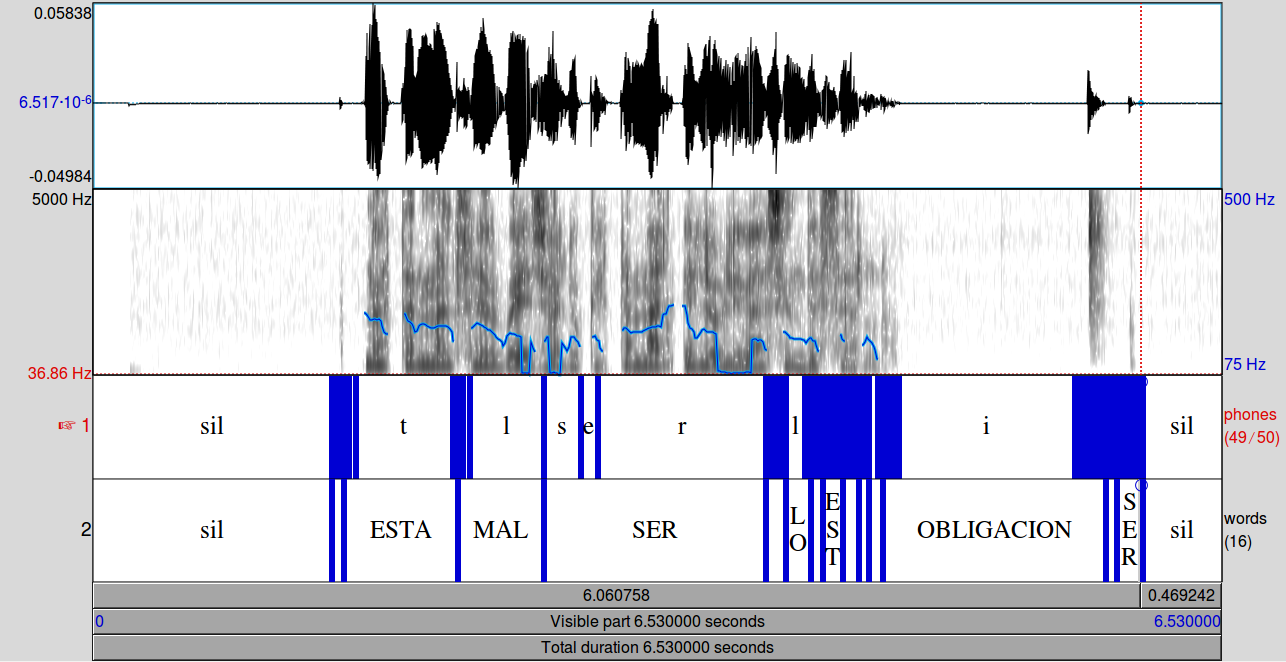
\includegraphics[width=0.8\textwidth]{alineacion_mala_inf} }
    \caption{Ejemplo de alineación mala por ruido}
    \label{alinMala}
\end{figure}

    \item \textbf{"Mouse clic" al finalizar:} las grabaciones recibieron ruido del movimiento propio del hablante. Pasó en muchas oportunidades que el clic de finalizar del mouse se grabó como parte final en el audio (Ver Figura \ref{clickFinal}). Ese sonido se grabó y afectó la alineación de forma tal que el alineador lo confunde con habla.
    
\begin{figure}[h!]
    \centerline{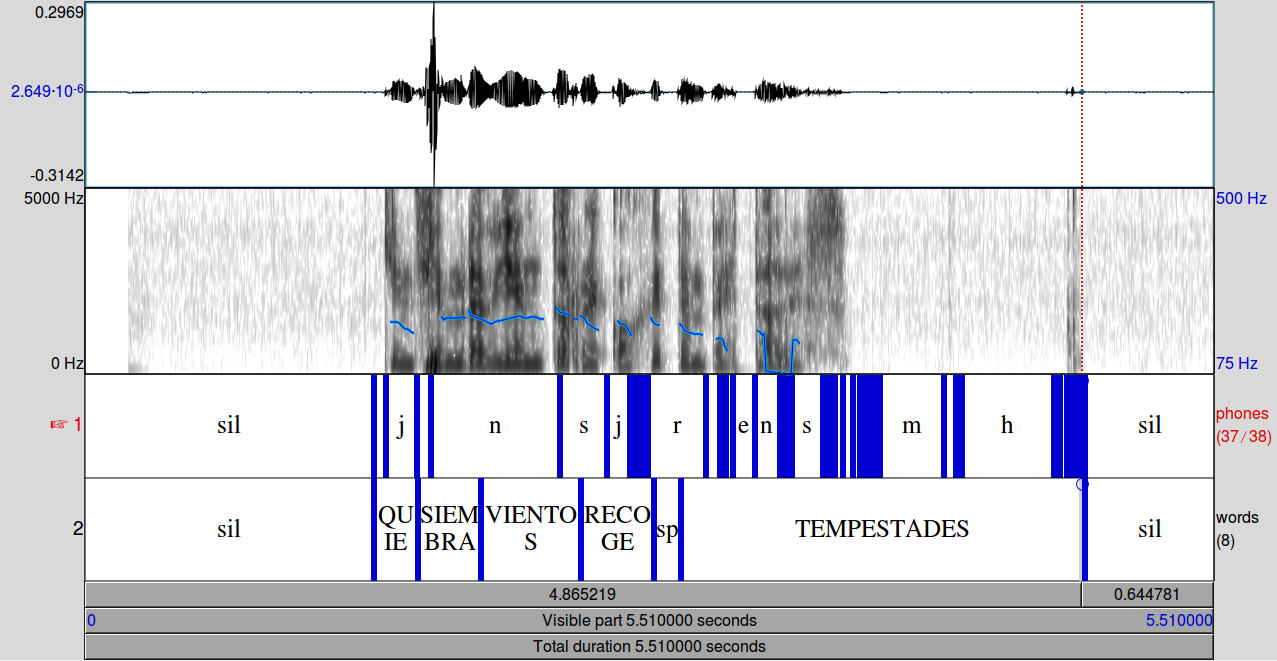
\includegraphics[width=0.8\textwidth]{click_al_final_inf} }
    \caption{Clic al final}
    \label{clickFinal}
\end{figure}

    \item \textbf{Saturación del micrófono:} el volumen del micrófono es configurado por el hablante. Es por ello que debemos confiar en su buena voluntad. Muchas veces la grabación fue buena pero en algunas partes la entonación tuvo mayor volumen que en otras; haciendo que, posteriormente, la alineación no sea precisa.
    
    \item \textbf{Entonación exagerada:} en algunas grabaciones se quiso exagerar la entonación. Por ejemplo, las palabras finalizadas en /s/ fueron grabadas en muchos casos sosteniendo ese fonema por tiempo prolongado. En la mayoría de los audios no sucedió, por lo que no afectó el análisis del experimento. El problema que surgió en estos casos fue que el hablante no supo pronunciar la frase de la forma más natural posible. 
    
\end{itemize}

\section{Corrección de errores}

%Corregir y explicar bien para qe se entiende la opcion de SCORES acá y en el capitulo anterior 
% ===> Llegué a la conclusión que mejor es no poner nada de SCORES en el documento y si decirlo en trabajos futuros
Para corregir los errores descriptos debimos chequear manualmente cada uno de los TextGrids. Los resultados de la cantidad de alineamientos corregidos se pueden ver en la tabla \ref{eva_table_align}.

%Esta tabla corresponde a los archivos en la carpeta ~/Tesis/Prosodylab-Aligner-master/data1.complete
\begin{table}[h]
\centering
\begin{tabular}{|l|c|c|c|c|}
\hline
\textbf{}  & \textbf{Bs.As. } & \textbf{Cba.} & \textbf{Total} \\ \hline
\textbf{Modificados}  & 101 & 88 & 189 \\ \hline
\textbf{Correctos}  & 119 & 2 & 121 \\ \hline
\textbf{Total} & 220 & 90 & 310 \\ \hline
\end{tabular}
\caption{Cantidad de alineamientos corregidos}
\label{eva_table_align}
\end{table}

Entonces las grabaciones que utilizamos salieron de estas 310 alineaciones. 

Recordemos que cada hablante tenía la posibilidad de grabar varias veces la misma frase con la idea de que la última grabación fuera la mejor grabada. Debemos quitar estos casos para no analizar frases que están mal grabadas. Contabilizamos los audios repetidos y los mostramos en la tabla \ref{eva_table_rep}.

\begin{table}[H]
\centering
\begin{tabular}{|l|c|c|c|}
\hline
\textbf{}  & \textbf{Bs.As. } & \textbf{Cba.} & \textbf{Total} \\ \hline
\textbf{Todos los intentos}  & 220 & 90 & 310 \\ \hline
\textbf{Último intento}  & \textbf{181} & \textbf{79} & \textbf{260} \\ \hline
\end{tabular}
\caption{Cantidad de audios repetidos}
\label{eva_table_rep}
\end{table}

Entonces los audios extraídos con la herramienta que vamos a utilizar para clasificar cada uno de los hablantes son: 181 audios para Buenos Aires y 79 audios para Córdoba.
En la próxima sección veremos el análisis que realizamos con estas grabaciones. 